\section{Transcodificador VP9 para AV1}
\label{cap:6.2}

No segundo trabalho desenvolvido no contexto desta tese, propusemos um transcodificador rápido de VP9 para AV1, ainda inédito na literatura. Neste trabalho, limitamos os tipos de particionamentos permitidos para serem testados no AV1 de acordo com o observado durante a decodificação do VP9, dependendo da profundidade atual da árvore no codificador AV1. A Figura \ref{fig:14}, apresentada no capítulo \ref{cap:4}, descreve os tipos de particionamentos que o formato AV1 permite, sendo eles: um quadrático (\textit{NONE}), dois binários retangulares (\textit{RECT}), quatro ternários mistos (\textit{AB}) e dois quaternários retangulares (\textit{1TO4}). Note que os tipos não-quadráticos possuem orientação horizontal e vertical. 

Como dito anteriormente, o AV1 é a evolução do formato de codificação de vídeo VP9. Portanto, herda deste diversas ferramentas de codificação. Enquanto o AV1 possui nove tipos de particionamento (capítulo \ref{cap:4}), o VP9 possui apenas três: quadrático, retangular orientado na vertical e retangular orientado na horizontal. Inclusive, há menos tamanhos quadráticos no VP9 (64$\times$64, 32$\times$32, 16$\times$16 e 8$\times$8), não sendo permitidos modos retangulares no menor tamanho. 

Com essas considerações, nesta proposta de transcodificador rápido de VP9 para AV1, avaliamos a correlação entre as orientações dos particionamentos aplicados no VP9 e as orientações dos particionamentos do AV1, para cada nível de profundidade e sob diferentes níveis de quantização.

\subsection{Metodologia}
\label{cap:6.2.1}

O primeiro passo deste trabalho foi correlacionar as orientações de particionamentos realizados pelos codificadores VP9 e AV1, considerando os quatro níveis de quantização utilizados pelas recomendações do AV1 \citet{bib:ietfnetvct}. Considerando quatro vídeos HD1080, foi possível obter as Tabelas \ref{tab:XI}, \ref{tab:XII}, \ref{tab:XIII} e \ref{tab:XIV}, que mostram essa correlação para os CQs 20, 32, 43 e 55, respectivamente, onde cada coluna totaliza 100\%. Como o AV1 possui mais tipos de particionamentos que o VP9, consideramos apenas as orientações horizontais ou verticais dos tipos \textit{AB} e \textit{1TO4}. As células em destaque nessas tabelas indicam quando os codificadores AV1 e VP9 escolhem a mesma profundidade e a mesma orientação de particionamento.

\afterpage{
\clearpage

\begin{landscape}
{\footnotesize

\begin{longtblr}[
    caption = {Correlação (em porcentagem) de orientação de particionamentos entre AV1 (linhas) e VP9 (colunas) por nível de profundidade (valores para o CQ 20).},
    label = {tab:XI}
]{
    colspec = {c|c|r|r|r|r|r|r|r|r|r|r},
    rowhead = 2,
    hlines,
    row{even} = {gray9},
    cell{7}{3}={cyan},
    cell{8}{4}={cyan},
    cell{9}{5}={cyan},
    cell{10}{6}={cyan},
    cell{11}{7}={cyan},
    cell{12}{8}={cyan},
    cell{13}{9}={cyan},
    cell{14}{10}={cyan},
    cell{15}{11}={cyan},
    cell{16}{12}={cyan}
}
\hline
\SetCell[c=2,r=2]{}& & \SetCell[c=10]{c} \textbf{VP9} &&&&&&&&\\
& & \SetCell[c=3]{c}\textbf{1 (64$\times$64)} &&& \SetCell[c=3]{c}\textbf{2 (32$\times$32)} &&& \SetCell[c=3]{c}\textbf{3 (16$\times$16)} &&& \textbf{4 (8$\times$8)} \\
\SetCell[c=2]{c} \textbf{AV1} && \textbf{Quad.} & \textbf{Horz.} & \textbf{Vert.} & \textbf{Quad.} & \textbf{Horz.} & \textbf{Vert.} & \textbf{Quad.} & \textbf{Horz.} & \textbf{Vert.} & \textbf{Quad.} \\
\SetCell[r=3]{c}\textbf{0 (128$\times$128)} & \textbf{Quad.} & 39,18 & 25,16 & 10,92 & 4,56 & 1,86 & 1,72 & 1,61 & 0,79 & 1,40 & 1,49 \\
 & \textbf{Horz.} & 1,15 & 0,38 & 0,39 & 0,16 & 0,06 & 0,06 & 0,04 & 0,12 & 0,01 & 0,03 \\
 & \textbf{Vert.} & 0,07 & 11,62 & 0,00 & 0,03 & 0,02 & 0,01 & 0,09 & 0,01 & 0,03 & 0,01 \\
\SetCell[r=3]{c}\textbf{1 (64$\times$64)} & \textbf{Quad.} & 36,93 & 15,36 & 30,23 & 12,54 & 5,02 & 4,92 & 3,48 & 2,36 & 2,97 & 5,58 \\
 & \textbf{Horz.} & 4,35 & 16,43 & 7,34 & 5,30 & 3,70 & 2,16 & 1,73 & 1,42 & 0,93 & 2,20 \\
 & \textbf{Vert.} & 6,21 & 5,25 & 17,55 & 5,82 & 1,78 & 3,57 & 1,41 & 0,90 & 1,17 & 2,01 \\
\SetCell[r=3]{c}\textbf{2 (32$\times$32)} & \textbf{Quad.} & 7,38 & 13,01 & 18,84 & 31,41 & 19,85 & 21,65 & 15,82 & 12,01 & 10,40 & 11,53 \\
 & \textbf{Horz.} & 1,62 & 6,01 & 4,32 & 13,32 & 25,30 & 13,42 & 16,45 & 15,73 & 9,73 & 10,97 \\
 & \textbf{Vert.} & 1,65 & 2,75 & 5,48 & 10,62 & 10,66 & 20,63 & 14,32 & 7,96 & 15,67 & 9,97 \\
\SetCell[r=3]{c}\textbf{3 (16$\times$16)} & \textbf{Quad.} & 0,83 & 2,17 & 2,65 & 8,52 & 15,77 & 16,33 & 22,78 & 17,48 & 21,09 & 17,19 \\
 & \textbf{Horz.} & 0,31 & 0,85 & 0,93 & 4,03 & 9,53 & 6,60 & 10,68 & 21,50 & 11,43 & 16,19 \\
 & \textbf{Vert.} & 0,24 & 0,71 & 0,99 & 2,79 & 4,64 & 7,16 & 8,82 & 8,64 & 18,87 & 13,23 \\
\SetCell[r=3]{c}\textbf{4 (8$\times$8)} & \textbf{Quad.} & 0,05 & 0,21 & 0,26 & 0,66 & 1,40 & 1,33 & 2,02 & 9,33 & 4,53 & 6,24 \\
 & \textbf{Horz.} & 0,01 & 0,05 & 0,05 & 0,13 & 0,25 & 0,21 & 0,38 & 1,08 & 0,67 & 1,65 \\
 & \textbf{Vert.} & 0,01 & 0,05 & 0,06 & 0,09 & 0,14 & 0,21 & 0,28 & 0,46 & 0,86 & 1,18 \\
\SetCell[r=1]{c}\textbf{5 (4$\times$4)} & \textbf{Quad.} & 0,00 & 0,00 & 0,01 & 0,02 & 0,04 & 0,04 & 0,07 & 0,19 & 0,22 & 0,52 \\
\hline
\end{longtblr}
}
\end{landscape}
}

\afterpage{
\clearpage

\begin{landscape}
{\footnotesize

\begin{longtblr}[
    caption = {Correlação (em porcentagem) de orientação de particionamentos entre AV1 (linhas) e VP9 (colunas) por nível de profundidade (valores para o CQ 32).},
    label = {tab:XII}
]{
    colspec = {c|c|r|r|r|r|r|r|r|r|r|r},
    rowhead = 2,
    hlines,
    row{even} = {gray9},
    cell{7}{3}={cyan},
    cell{8}{4}={cyan},
    cell{9}{5}={cyan},
    cell{10}{6}={cyan},
    cell{11}{7}={cyan},
    cell{12}{8}={cyan},
    cell{13}{9}={cyan},
    cell{14}{10}={cyan},
    cell{15}{11}={cyan},
    cell{16}{12}={cyan}
}
\hline
\SetCell[c=2,r=2]{}& & \SetCell[c=10]{c} \textbf{VP9} &&&&&&&&\\
& & \SetCell[c=3]{c}\textbf{1 (64$\times$64)} &&& \SetCell[c=3]{c}\textbf{2 (32$\times$32)} &&& \SetCell[c=3]{c}\textbf{3 (16$\times$16)} &&& \textbf{4 (8$\times$8)} \\
\SetCell[c=2]{c} \textbf{AV1} && \textbf{Quad.} & \textbf{Horz.} & \textbf{Vert.} & \textbf{Quad.} & \textbf{Horz.} & \textbf{Vert.} & \textbf{Quad.} & \textbf{Horz.} & \textbf{Vert.} & \textbf{Quad.} \\
\SetCell[r=3]{c}\textbf{0 (128$\times$128)} & \textbf{Quad.} & 51,60 & 26,07 & 8,27 & 5,26 & 2,85 & 2,77 & 2,74 & 1,04 & 1,64 & 2,64 \\
 & \textbf{Horz.} & 1,48 & 0,46 & 0,38 & 0,24 & 0,10 & 0,10 & 0,07 & 0,15 & 0,01 & 0,06 \\
 & \textbf{Vert.} & 0,23 & 13,47 & 0,00 & 0,06 & 0,03 & 0,03 & 0,22 & 0,02 & 0,03 & 0,27 \\
\SetCell[r=3]{c}\textbf{1 (64$\times$64)} & \textbf{Quad.} & 27,28 & 14,02 & 26,20 & 11,92 & 5,83 & 5,03 & 5,44 & 4,11 & 5,02 & 9,91 \\
 & \textbf{Horz.} & 3,32 & 11,73 & 6,06 & 6,30 & 5,30 & 2,50 & 2,79 & 2,02 & 1,62 & 3,05 \\
 & \textbf{Vert.} & 4,41 & 4,42 & 16,74 & 6,92 & 2,83 & 4,93 & 2,98 & 1,55 & 2,19 & 3,19 \\
\SetCell[r=3]{c}\textbf{2 (32$\times$32)} & \textbf{Quad.} & 6,56 & 14,77 & 21,18 & 34,00 & 22,50 & 26,26 & 20,19 & 17,56 & 15,13 & 15,27 \\
 & \textbf{Horz.} & 1,83 & 6,18 & 5,92 & 11,60 & 25,49 & 11,20 & 15,15 & 15,83 & 9,36 & 10,30 \\
 & \textbf{Vert.} & 1,51 & 3,48 & 7,55 & 10,22 & 9,16 & 19,76 & 13,61 & 8,31 & 16,27 & 9,99 \\
\SetCell[r=3]{c}\textbf{3 (16$\times$16)} & \textbf{Quad.} & 0,92 & 3,07 & 4,35 & 7,66 & 13,56 & 14,37 & 20,40 & 15,34 & 18,63 & 14,00 \\
 & \textbf{Horz.} & 0,44 & 1,27 & 1,52 & 2,98 & 7,48 & 4,99 & 7,59 & 18,29 & 9,58 & 13,49 \\
 & \textbf{Vert.} & 0,31 & 0,79 & 1,47 & 2,24 & 3,40 & 6,56 & 6,62 & 6,69 & 15,16 & 10,21 \\
\SetCell[r=3]{c}\textbf{4 (8$\times$8)} & \textbf{Quad.} & 0,07 & 0,20 & 0,26 & 0,47 & 1,11 & 1,14 & 1,61 & 7,42 & 3,84 & 4,90 \\
 & \textbf{Horz.} & 0,02 & 0,04 & 0,06 & 0,07 & 0,21 & 0,13 & 0,30 & 1,01 & 0,64 & 1,34 \\
 & \textbf{Vert.} & 0,01 & 0,02 & 0,04 & 0,06 & 0,09 & 0,18 & 0,23 & 0,45 & 0,69 & 0,97 \\
\SetCell[r=1]{c}\textbf{5 (4$\times$4)} & \textbf{Quad.} & 0,00 & 0,00 & 0,01 & 0,01 & 0,03 & 0,03 & 0,07 & 0,21 & 0,18 & 0,42 \\
\hline
\end{longtblr}
}
\end{landscape}
}

\afterpage{
\clearpage

\begin{landscape}
{\footnotesize

\begin{longtblr}[
    caption = {Correlação (em porcentagem) de orientação de particionamentos entre AV1 (linhas) e VP9 (colunas) por nível de profundidade (valores para o CQ 43).},
    label = {tab:XIII}
]{
    colspec = {c|c|r|r|r|r|r|r|r|r|r|r},
    rowhead = 2,
    hlines,
    row{even} = {gray9},
    cell{7}{3}={cyan},
    cell{8}{4}={cyan},
    cell{9}{5}={cyan},
    cell{10}{6}={cyan},
    cell{11}{7}={cyan},
    cell{12}{8}={cyan},
    cell{13}{9}={cyan},
    cell{14}{10}={cyan},
    cell{15}{11}={cyan},
    cell{16}{12}={cyan}
}
\hline
\SetCell[c=2,r=2]{}& & \SetCell[c=10]{c} \textbf{VP9} &&&&&&&&\\
& & \SetCell[c=3]{c}\textbf{1 (64$\times$64)} &&& \SetCell[c=3]{c}\textbf{2 (32$\times$32)} &&& \SetCell[c=3]{c}\textbf{3 (16$\times$16)} &&& \textbf{4 (8$\times$8)} \\
\SetCell[c=2]{c} \textbf{AV1} && \textbf{Quad.} & \textbf{Horz.} & \textbf{Vert.} & \textbf{Quad.} & \textbf{Horz.} & \textbf{Vert.} & \textbf{Quad.} & \textbf{Horz.} & \textbf{Vert.} & \textbf{Quad.} \\
\SetCell[r=3]{c}\textbf{0 (128$\times$128)} & \textbf{Quad.} & 52,23 & 24,66 & 8,86 & 6,60 & 2,99 & 1,92 & 4,72 & 3,45 & 3,99 & 6,82 \\
 & \textbf{Horz.} & 1,55 & 0,41 & 0,42 & 0,37 & 0,03 & 0,05 & 0,04 & 0,12 & 0,00 & 0,02 \\
 & \textbf{Vert.} & 0,39 & 14,63 & 0,03 & 0,08 & 0,03 & 0,06 & 0,26 & 0,08 & 0,08 & 0,22 \\
\SetCell[r=3]{c}\textbf{1 (64$\times$64)} & \textbf{Quad.} & 26,70 & 15,33 & 27,79 & 16,26 & 10,52 & 9,77 & 12,15 & 9,67 & 10,78 & 16,36 \\
 & \textbf{Horz.} & 3,34 & 13,51 & 6,95 & 8,90 & 10,50 & 5,05 & 5,35 & 5,40 & 3,08 & 4,45 \\
 & \textbf{Vert.} & 4,41 & 4,99 & 17,74 & 8,75 & 4,65 & 10,04 & 5,25 & 2,93 & 5,14 & 3,78 \\
\SetCell[r=3]{c}\textbf{2 (32$\times$32)} & \textbf{Quad.} & 6,41 & 14,31 & 20,89 & 34,15 & 23,95 & 28,20 & 21,81 & 23,18 & 18,55 & 17,07 \\
 & \textbf{Horz.} & 1,72 & 5,56 & 4,92 & 7,69 & 21,75 & 8,32 & 11,70 & 13,73 & 7,25 & 8,20 \\
 & \textbf{Vert.} & 1,35 & 2,33 & 6,60 & 7,50 & 6,15 & 16,08 & 10,78 & 5,90 & 13,49 & 8,24 \\
\SetCell[r=3]{c}\textbf{3 (16$\times$16)} & \textbf{Quad.} & 1,04 & 2,45 & 3,37 & 5,66 & 10,72 & 11,57 & 16,74 & 12,09 & 15,59 & 10,88 \\
 & \textbf{Horz.} & 0,44 & 1,08 & 1,03 & 2,02 & 5,25 & 3,41 & 5,22 & 13,67 & 6,99 & 10,82 \\
 & \textbf{Vert.} & 0,34 & 0,54 & 1,16 & 1,59 & 2,35 & 4,44 & 4,48 & 4,45 & 11,14 & 7,92 \\
\SetCell[r=3]{c}\textbf{4 (8$\times$8)} & \textbf{Quad.} & 0,06 & 0,17 & 0,17 & 0,34 & 0,81 & 0,86 & 1,11 & 4,30 & 2,89 & 3,25 \\
 & \textbf{Horz.} & 0,01 & 0,03 & 0,03 & 0,05 & 0,22 & 0,10 & 0,20 & 0,62 & 0,40 & 1,03 \\
 & \textbf{Vert.} & 0,01 & 0,01 & 0,03 & 0,04 & 0,07 & 0,12 & 0,14 & 0,28 & 0,47 & 0,68 \\
\SetCell[r=1]{c}\textbf{5 (4$\times$4)} & \textbf{Quad.} & 0,00 & 0,00 & 0,00 & 0,01 & 0,02 & 0,02 & 0,04 & 0,13 & 0,15 & 0,26 \\
\hline
\end{longtblr}
}
\end{landscape}
}

\afterpage{
\clearpage

\begin{landscape}
{\footnotesize

\begin{longtblr}[
    caption = {Correlação (em porcentagem) de orientação de particionamentos entre AV1 (linhas) e VP9 (colunas) por nível de profundidade (valores para o CQ 55).},
    label = {tab:XIV}
]{
    colspec = {c|c|r|r|r|r|r|r|r|r|r|r},
    rowhead = 2,
    hlines,
    row{even} = {gray9},
    cell{7}{3}={cyan},
    cell{8}{4}={cyan},
    cell{9}{5}={cyan},
    cell{10}{6}={cyan},
    cell{11}{7}={cyan},
    cell{12}{8}={cyan},
    cell{13}{9}={cyan},
    cell{14}{10}={cyan},
    cell{15}{11}={cyan},
    cell{16}{12}={cyan}
}
\hline
\SetCell[c=2,r=2]{}& & \SetCell[c=10]{c} \textbf{VP9} &&&&&&&&\\
& & \SetCell[c=3]{c}\textbf{1 (64$\times$64)} &&& \SetCell[c=3]{c}\textbf{2 (32$\times$32)} &&& \SetCell[c=3]{c}\textbf{3 (16$\times$16)} &&& \textbf{4 (8$\times$8)} \\
\SetCell[c=2]{c} \textbf{AV1} && \textbf{Quad.} & \textbf{Horz.} & \textbf{Vert.} & \textbf{Quad.} & \textbf{Horz.} & \textbf{Vert.} & \textbf{Quad.} & \textbf{Horz.} & \textbf{Vert.} & \textbf{Quad.} \\
\SetCell[r=3]{c}\textbf{0 (128$\times$128)} & \textbf{Quad.} & 55,85 & 25,00 & 12,99 & 10,91 & 7,60 & 4,40 & 9,64 & 9,52 & 10,84 & 10,20 \\
 & \textbf{Horz.} & 1,62 & 0,50 & 0,72 & 0,39 & 0,10 & 0,07 & 0,16 & 0,44 & 0,10 & 0,26 \\
 & \textbf{Vert.} & 0,44 & 17,05 & 0,03 & 0,25 & 0,08 & 0,64 & 0,43 & 0,07 & 0,31 & 0,21 \\
\SetCell[r=3]{c}\textbf{1 (64$\times$64)} & \textbf{Quad.} & 27,07 & 18,28 & 33,51 & 26,73 & 22,43 & 21,70 & 21,62 & 18,89 & 19,88 & 20,50 \\
 & \textbf{Horz.} & 2,79 & 15,70 & 5,92 & 9,41 & 14,52 & 5,94 & 7,50 & 9,47 & 4,92 & 6,56 \\
 & \textbf{Vert.} & 3,29 & 2,91 & 16,52 & 8,16 & 4,01 & 11,55 & 6,00 & 4,08 & 8,61 & 5,21 \\
\SetCell[r=3]{c}\textbf{2 (32$\times$32)} & \textbf{Quad.} & 5,08 & 11,68 & 17,91 & 27,77 & 20,04 & 25,30 & 19,20 & 19,76 & 17,36 & 16,24 \\
 & \textbf{Horz.} & 1,33 & 4,33 & 3,19 & 5,34 & 15,61 & 5,88 & 9,36 & 11,12 & 6,29 & 7,18 \\
 & \textbf{Vert.} & 1,01 & 1,68 & 5,38 & 5,13 & 3,91 & 12,65 & 8,52 & 5,23 & 10,24 & 7,17 \\
\SetCell[r=3]{c}\textbf{3 (16$\times$16)} & \textbf{Quad.} & 0,87 & 1,72 & 2,40 & 3,64 & 6,68 & 7,27 & 11,30 & 8,83 & 9,49 & 8,51 \\
 & \textbf{Horz.} & 0,32 & 0,70 & 0,46 & 1,08 & 3,37 & 1,66 & 3,06 & 7,72 & 3,95 & 8,02 \\
 & \textbf{Vert.} & 0,25 & 0,35 & 0,87 & 0,94 & 1,07 & 2,47 & 2,54 & 2,98 & 6,22 & 6,00 \\
\SetCell[r=3]{c}\textbf{4 (8$\times$8)} & \textbf{Quad.} & 0,05 & 0,08 & 0,07 & 0,18 & 0,41 & 0,37 & 0,48 & 1,45 & 1,30 & 2,37 \\
 & \textbf{Horz.} & 0,01 & 0,01 & 0,01 & 0,03 & 0,10 & 0,05 & 0,10 & 0,28 & 0,19 & 0,83 \\
 & \textbf{Vert.} & 0,01 & 0,01 & 0,02 & 0,03 & 0,04 & 0,05 & 0,08 & 0,15 & 0,26 & 0,58 \\
\SetCell[r=1]{c}\textbf{5 (4$\times$4)} & \textbf{Quad.} & 0,00 & 0,00 & 0,00 & 0,01 & 0,01 & 0,00 & 0,01 & 0,02 & 0,03 & 0,17 \\
\hline
\end{longtblr}

}
\end{landscape}
}


Considerando essas tabelas, torna-se possível identificar qual é a maior probabilidade de ocorrer alguma orientação de particionamento no transcodificador para AV1, dadas as observações no decodificador VP9. Essas orientações mais comuns são mostradas para cada uma das profundidades disponíveis no AV1 e para todos os níveis de quantização utilizados. É possível compreender melhor essas tabelas através do seguinte exemplo: em uma determinada região do vídeo, identifiquemos que o codificador VP9 optou por utilizar o segundo nível de profundidade, havendo dois blocos 32$\times$16, ou seja, com orientação vertical. Ao observarmos a codificação do AV1 no CQ 43 (Tabela \ref{tab:XIII}), há uma probabilidade inferior a 2\% de que o codificador AV1 opte por utilizar uma profundidade 0 com orientação quadrática (bloco 128$\times$128) nessa mesma região do vídeo. Contudo, no terceiro nível de profundidade, o codificador AV1 vai optar por utilizar a orientação quadrática em 28\% das vezes e, em seguida, a orientação vertical em 16\% das vezes. Observações semelhantes podem ser feitas para as quatro tabelas de correlação apresentadas.

Com essas correlações estabelecidas, determinamos que o codificador AV1 somente pode testar blocos orientados de acordo com as maiores probabilidades de orientação observadas nas Tabelas \ref{tab:XI}, \ref{tab:XII}, \ref{tab:XIII} e \ref{tab:XIV}. É possível resumir essas tabelas através da Tabela \ref{tab:XV}, onde destacam-se as únicas orientações autorizadas a serem testadas no codificador AV1, dadas a profundidade atual na codificação e a orientação observada no formato VP9. Note que a profundidade 5 do AV1 possui apenas orientação quadrática, razão pela qual ela não está presente na Tabela \ref{tab:XV}. Como podemos observar, quase todas as probabilidades de escolha do codificador AV1 tendem para a orientação quadrática. Dessa forma, é possível definir um pseudocódigo que simplifica a Tabela \ref{tab:XV}, como apresentado na Figura \ref{fig:23}. Através desse pseudocódigo, podemos apresentar a proposta de transcodificador rápido do formato VP9 para AV1, como consta na Figura \ref{fig:24}.

\afterpage{
\clearpage

\begin{landscape}
{\footnotesize
\begin{longtblr}[
    caption = {Resumo de particionamentos permitidos ao codificador AV1, de acordo com as Tabelas \ref{tab:XI}, \ref{tab:XII}, \ref{tab:XIII} e \ref{tab:XIV}. Destacou-se as células que não são Quad.},
    label = {tab:XV}
]{
    colspec = {l|l|c|l|l|l|l|l|l|l|l|l|l},
    rowhead = 3,
    hlines,
    row{even} = {gray9},
    cell{2}{1}={white},
    cell{4}{1}={white},
    cell{5}{5}={cyan},
    cell{6}{8}={cyan},
    cell{6}{10}={cyan},
    cell{6}{11}={cyan},
    cell{6}{12}={cyan},
    cell{7}{11}={cyan},
    cell{11}{8}={cyan},
    cell{11}{10}={cyan},
    cell{11}{11}={cyan},
    cell{11}{12}={cyan},
    cell{12}{11}={cyan},
    cell{15}{6}={cyan},
    cell{17}{11}={cyan},
}
\hline
\SetCell[c=3]{c} &&& \SetCell[c=10]{c} \textbf{Profundidade e Orientação Observadas no VP9}\\
\SetCell[c=2,r=2]{c} && \SetCell[r=2]{c}\textbf{Profundidade} & \SetCell[c=3]{c}\textbf{1} &&& \SetCell[c=3]{c}\textbf{2} &&& \SetCell[c=3]{c}\textbf{3} &&& \textbf{4} \\
&&& \textbf{Quad.} & \textbf{Horz.} & \textbf{Vert.} & \textbf{Quad.} & \textbf{Horz.} & \textbf{Vert.} & \textbf{Quad.} & \textbf{Horz.} & \textbf{Vert.} & \textbf{Quad.} \\
\SetCell[r=17]{c}\rotatebox{90}{\textbf{Condição do Bloco no AV1}} & \SetCell[r=5]{c}\textbf{CQ 20} & \textbf{0} & Quad. & Quad. & Quad. & Quad. & Quad. & Quad. & Quad. & Quad. & Quad. & Quad. \\
 & & \textbf{1} & Quad. & Horz. & Quad. & Quad. & Quad. & Quad. & Quad. & Quad. & Quad. & Quad. \\
 & & \textbf{2} & Quad. & Quad. & Quad. & Quad. & Horz. & Quad. & Horz. & Horz. & Vert. & Quad. \\
 & & \textbf{3} & Quad. & Quad. & Quad. & Quad. & Quad. & Quad. & Quad. & Horz. & Quad. & Quad. \\
 & & \textbf{4} & Quad. & Quad. & Quad. & Quad. & Quad. & Quad. & Quad. & Quad. & Quad. & Quad. \\
 & \SetCell[r=5]{c}\textbf{CQ 32} & \textbf{0} & Quad. & Quad. & Quad. & Quad. & Quad. & Quad. & Quad. & Quad. & Quad. & Quad. \\
 & & \textbf{1} & Quad. & Quad. & Quad. & Quad. & Quad. & Quad. & Quad. & Quad. & Quad. & Quad. \\
 & & \textbf{2} & Quad. & Quad. & Quad. & Quad. & Horz. & Quad. & Horz. & Horz. & Vert. & Quad. \\
 & & \textbf{3} & Quad. & Quad. & Quad. & Quad. & Quad. & Quad. & Quad. & Horz. & Quad. & Quad. \\
 & & \textbf{4} & Quad. & Quad. & Quad. & Quad. & Quad. & Quad. & Quad. & Quad. & Quad. & Quad. \\
 & \SetCell[r=5]{c}\textbf{CQ 43} & \textbf{0} & Quad. & Quad. & Quad. & Quad. & Quad. & Quad. & Quad. & Quad. & Quad. & Quad. \\
 & & \textbf{1} & Quad. & Quad. & Vert. & Quad. & Quad. & Quad. & Quad. & Quad. & Quad. & Quad. \\
 & & \textbf{2} & Quad. & Quad. & Quad. & Quad. & Quad. & Quad. & Quad. & Quad. & Quad. & Quad. \\
 & & \textbf{3} & Quad. & Quad. & Quad. & Quad. & Quad. & Quad. & Quad. & Horz. & Quad. & Quad. \\
 & & \textbf{4} & Quad. & Quad. & Quad. & Quad. & Quad. & Quad. & Quad. & Quad. & Quad. & Quad. \\
 & \SetCell[r=2]{c}\textbf{CQ 55} & \textbf{0} & Quad. & Quad. & Quad. & Quad. & Quad. & Quad. & Quad. & Quad. & Quad. & Quad. \\
 & & \textbf{1} & Quad. & Quad. & Quad. & Quad. & Quad. & Quad. & Quad. & Quad. & Quad. & Quad. \\
\SetCell[r=3]{c} & \SetCell[r=3]{c}\textbf{CQ 55} & \textbf{2} & Quad. & Quad. & Quad. & Quad. & Quad. & Quad. & Quad. & Quad. & Quad. & Quad. \\
& & \textbf{3} & Quad. & Quad. & Quad. & Quad. & Quad. & Quad. & Quad. & Quad. & Quad. & Quad. \\
 & & \textbf{4} & Quad. & Quad. & Quad. & Quad. & Quad. & Quad. & Quad. & Quad. & Quad. & Quad. \\
\hline
\end{longtblr}
}
\end{landscape}
}



\begin{figure}
    \centering
    \footnotesize
    %\includegraphics[width=0.75\textwidth,trim=4 4 4 4,clip]{ChapterSIX/figs/fig23.png}
    \begin{Verbatim}[frame=single,commandchars=\\\{\}]
        orientacaoAV1 <- \textcolor{red}{Quad.}
	\textcolor{blue}{se} profundidadeAV1 \textcolor{blue}{for} 1 \textcolor{blue}{faça}:
		\textcolor{blue}{se} profundidadeVP9 \textcolor{blue}{for} 1 
			\textcolor{blue}{e} orientacaoVP9 \textcolor{blue}{for} Horz. 
			\textcolor{blue}{e} quantização \textcolor{blue}{for} 20 \textcolor{blue}{faça}:
				orientacaoAV1 <- \textcolor{red}{Horz.}
		\textcolor{blue}{se} profundidadeVP9 \textcolor{blue}{for} 2 
			\textcolor{blue}{e} orientacaoVP9 \textcolor{blue}{for} Vert. 
			\textcolor{blue}{e} quantização \textcolor{blue}{for} 43 \textcolor{blue}{faça}:
				orientacaoAV1 <- \textcolor{red}{Vert.}
	\textcolor{blue}{se} profundidadeAV1 \textcolor{blue}{for} 2 \textcolor{blue}{faça}:
		\textcolor{blue}{se} profundidadeVP9 \textcolor{blue}{for} 2 
			\textcolor{blue}{e} orientacaoVP9 \textcolor{blue}{for} Horz. 
			\textcolor{blue}{e} quantização \textcolor{blue}{for} 20 \textcolor{blue}{faça}:
				orientacaoAV1 <- \textcolor{red}{Horz.}
		\textcolor{blue}{se} profundidadeVP9 \textcolor{blue}{for} 2 
			\textcolor{blue}{e} orientacaoVP9 \textcolor{blue}{for} Horz. 
			\textcolor{blue}{e} quantização \textcolor{blue}{for} 32 \textcolor{blue}{faça}:
				orientacaoAV1 <- \textcolor{red}{Horz.}
		\textcolor{blue}{se} profundidadeVP9 \textcolor{blue}{for} 3 
			\textcolor{blue}{e} orientacaoVP9 \textcolor{blue}{for} Quad. 
			\textcolor{blue}{e} quantização \textcolor{blue}{for} 20 \textcolor{blue}{faça}:
				orientacaoAV1 <- \textcolor{red}{Horz.}
		\textcolor{blue}{se} profundidadeVP9 \textcolor{blue}{for} 3 
			\textcolor{blue}{e} orientacaoVP9 \textcolor{blue}{for} Horz. 
			\textcolor{blue}{e} quantização \textcolor{blue}{for} 20 \textcolor{blue}{faça}:
				orientacaoAV1 <- \textcolor{red}{Horz.}
		\textcolor{blue}{se} profundidadeVP9 \textcolor{blue}{for} 3 
			\textcolor{blue}{e} orientacaoVP9 \textcolor{blue}{for} Vert. 
			\textcolor{blue}{e} quantização \textcolor{blue}{for} 20 \textcolor{blue}{faça}:
				orientacaoAV1 <- \textcolor{red}{Vert.}
		\textcolor{blue}{se} profundidadeVP9 \textcolor{blue}{for} 3 
			\textcolor{blue}{e} orientacaoVP9 \textcolor{blue}{for} Vert. 
			\textcolor{blue}{e} quantização \textcolor{blue}{for} 32 \textcolor{blue}{faça}:
				orientacaoAV1 <- \textcolor{red}{Vert.}
	\textcolor{blue}{se} profundidadeAV1 \textcolor{blue}{for} 3 \textcolor{blue}{faça}:
		\textcolor{blue}{se} profundidadeVP9 \textcolor{blue}{for} 3 
			\textcolor{blue}{e} orientacaoVP9 \textcolor{blue}{for} Horz. 
			\textcolor{blue}{e} quantização \textcolor{blue}{for} 20 \textcolor{blue}{faça}:
				orientacaoAV1 <- \textcolor{red}{Horz.}
		\textcolor{blue}{se} profundidadeVP9 \textcolor{blue}{for} 3 
			\textcolor{blue}{e} orientacaoVP9 \textcolor{blue}{for} Horz. 
			\textcolor{blue}{e} quantização \textcolor{blue}{for} 32 \textcolor{blue}{faça}:
				orientacaoAV1 <- \textcolor{red}{Horz.}
		\textcolor{blue}{se} profundidadeVP9 \textcolor{blue}{for} 3 
			\textcolor{blue}{e} orientacaoVP9 \textcolor{blue}{for} Horz. 
			\textcolor{blue}{e} quantização \textcolor{blue}{for} 43 \textcolor{blue}{faça}:
				orientacaoAV1 <- \textcolor{red}{Horz.}
	\textcolor{blue}{retorna} orientacaoAV1
    \end{Verbatim}
    \caption{Pseudocódigo implementado no AV1 para escolha de orientação de particionamentos, baseado na Tabela \ref{tab:XV}. Fonte: Elaborada pelo autor.}
    \label{fig:23}
\end{figure}

\begin{figure}
    \centering
    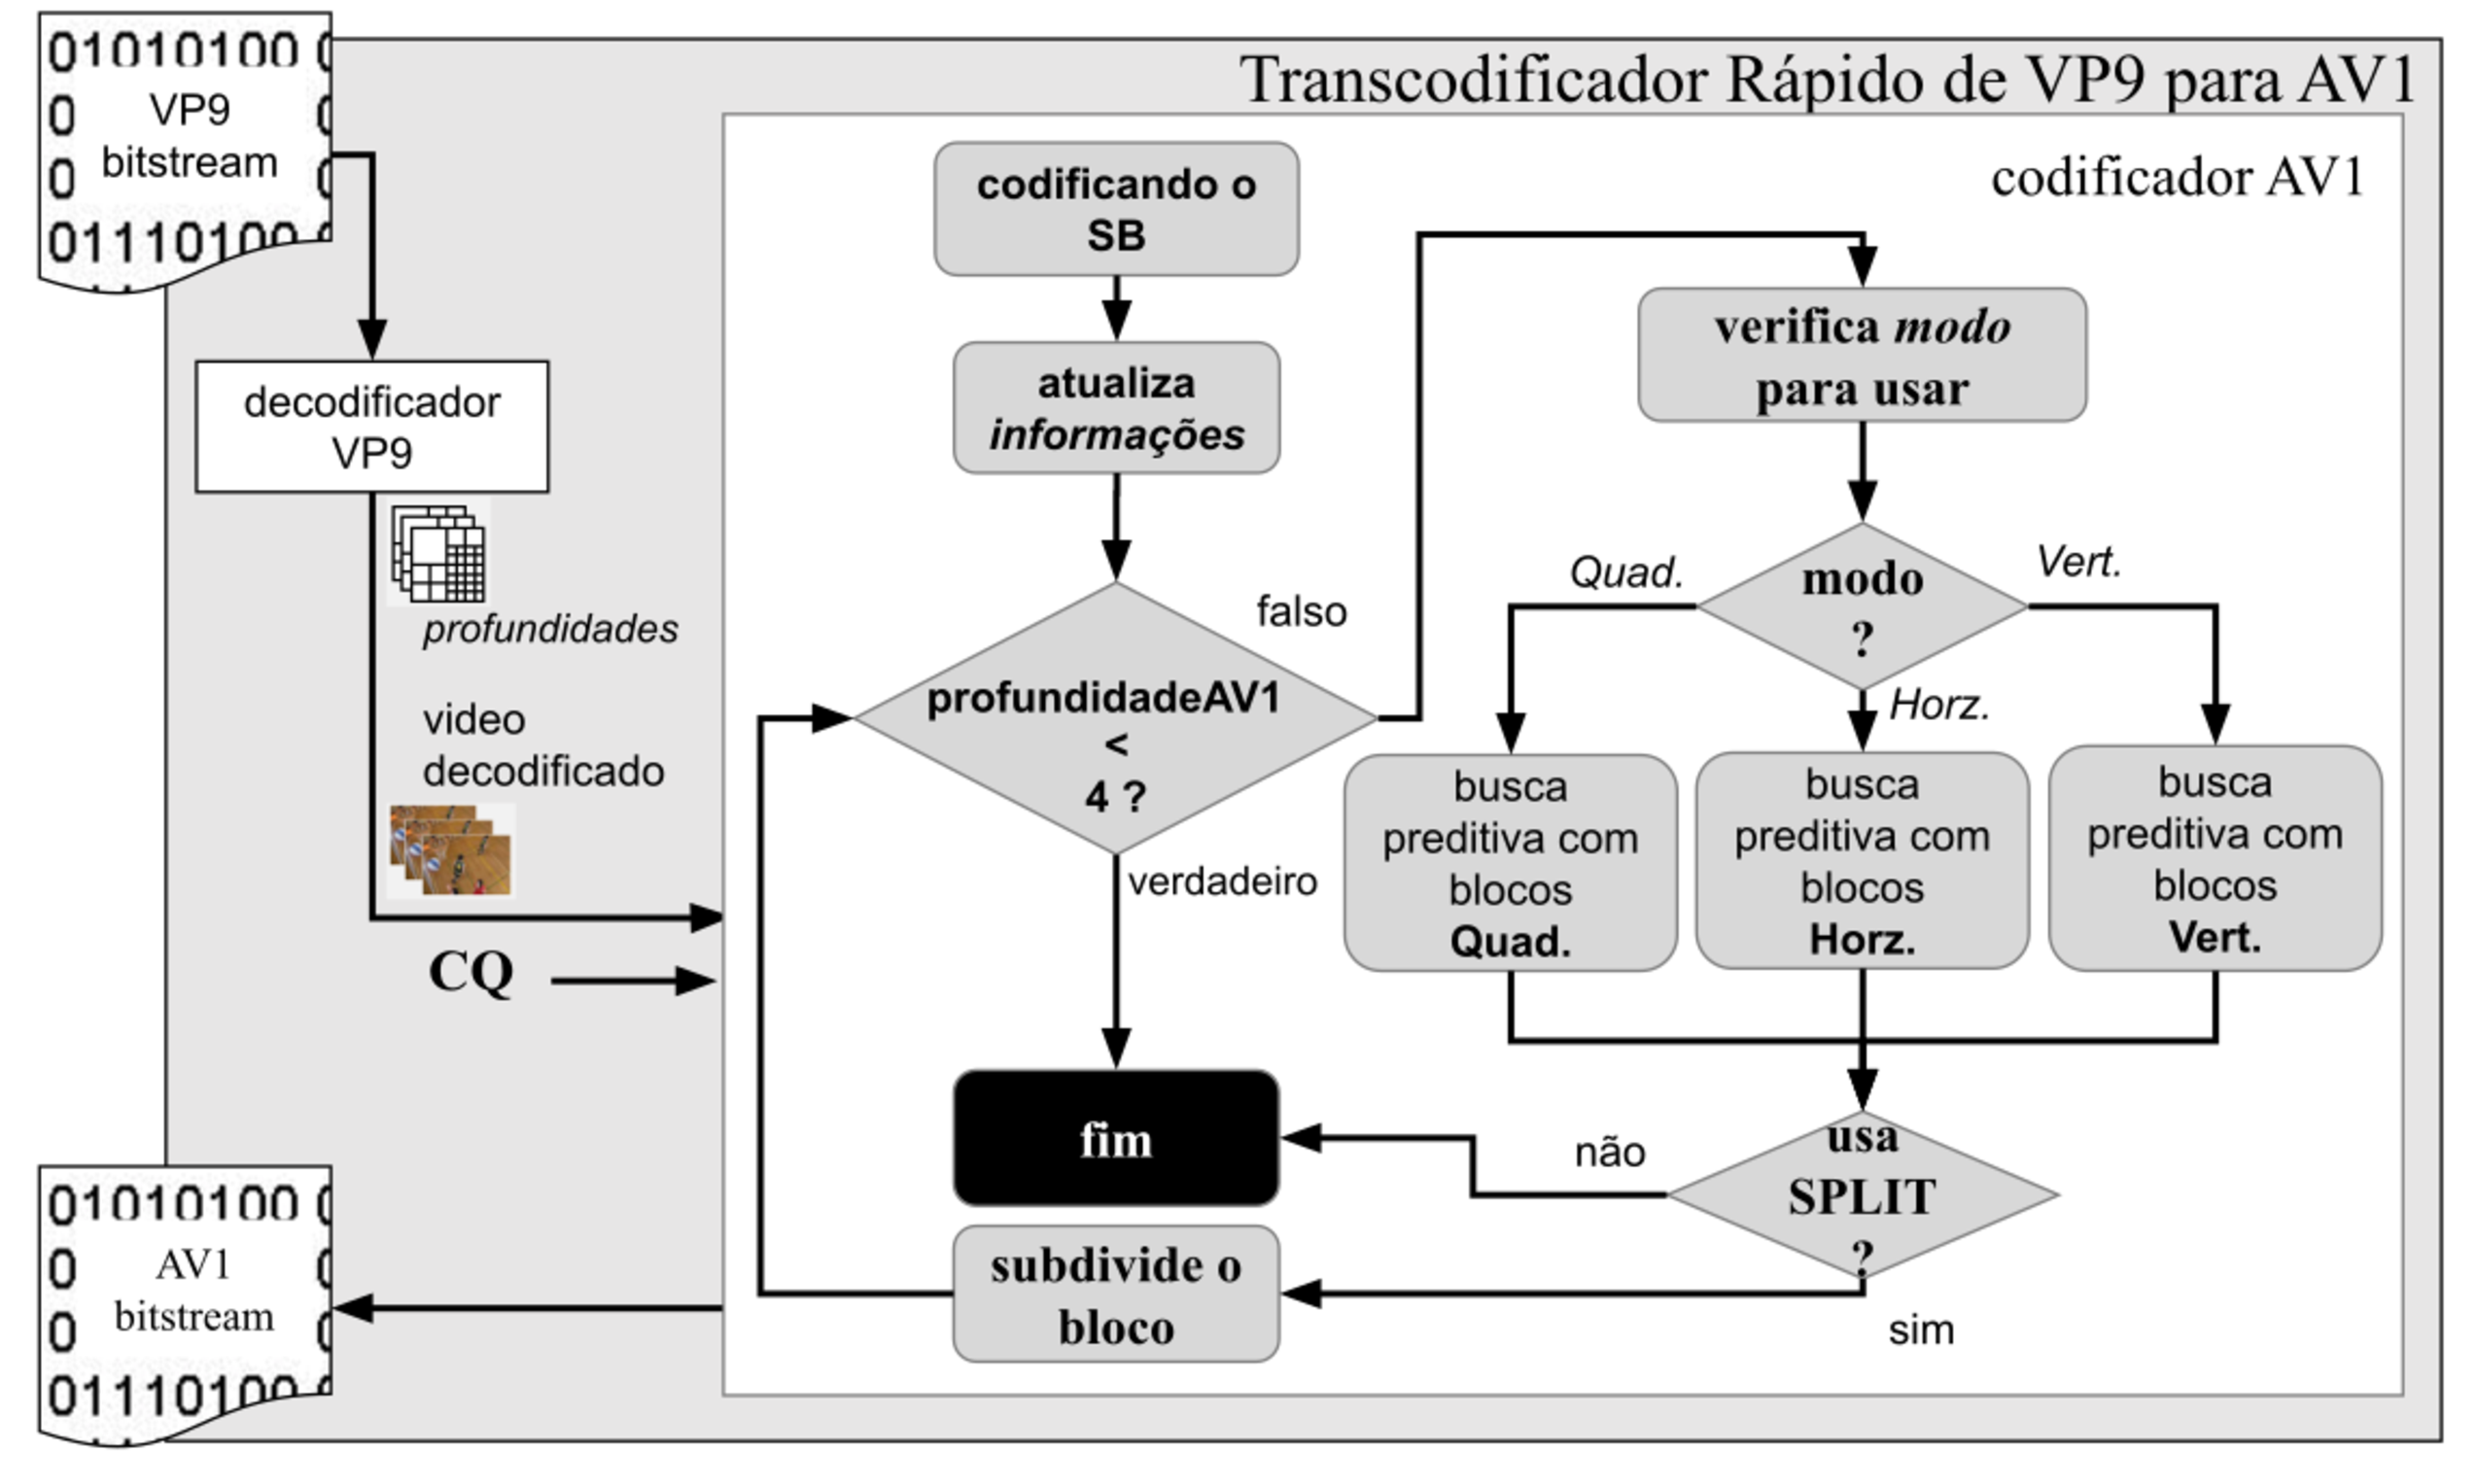
\includegraphics[width=0.85\textwidth]{FIGURES/fig_24.png}
    \caption{Proposta de transcodificação rápida do formato VP9 para AV1 baseada em análises estatísticas. Fonte: Elaborada pelo autor.}
    \label{fig:24}
\end{figure}

O algoritmo representado no fluxograma da Figura \ref{fig:24} tem como entrada informações do decodificador, indicando as profundidades e orientações de cada árvore de particionamentos decodificada. Durante a execução do codificador, informações sobre o nível de quantização utilizado e o nível atual da árvore são utilizados para avaliar a correta orientação a ser utilizada naquele ponto do vídeo. A única exceção é caso a profundidade atual seja igual a cinco, como representado no primeiro condicional da Figura \ref{fig:24}. 

\subsection{Resultados}
\label{cap:6.2.2}

Para possibilitar a realização dos experimentos de avaliação deste transcodificador rápido, foram utilizados 60 quadros de 20 sequências de vídeos em diversas resoluções, separadas em categorias de resolução. Com isso, foi possível obter os resultados apresentados na Tabela \ref{tab:XVI}, onde se observa uma redução média de 28,16\% do tempo total da transcodificação em relação à transcodificação original, a um custo de elevar o BD-rate em 4,34\%.

\afterpage{
\clearpage

\begin{landscape}
{\footnotesize
\begin{longtblr}[
    caption = {Resultados da transcodificação rápida de VP9 para AV1 baseada em análise estatística.},
    label = {tab:XVI}
]{
    colspec = {l|l|r|r|r},
    rowhead = 1,
    hlines,
    row{even} = {gray9}
}
\hline

\textbf{Classe} & \textbf{Sequência} & \textbf{BD-rate (\%)} & \textbf{TS (\%)} & \textbf{Razão} \\
\SetCell[r=4]{l}CIF & bqfree\_240p\_120f & 4,7555 & 24,18 & 0,197 \\
 & bqzoom\_240p\_120f & 4,4228 & 23,37 & 0,189 \\
 & chairlift\_240p\_120f & 4,0765 & 26,89 & 0,152 \\
 & mozzoom\_240p\_120f & 2,7979 & 26,15 & 0,107 \\
\SetCell[c=2]{r}Média – CIF && 4,0132 & 25,15 & \\
\SetCell[c=2]{r}Desvio Padrão – CIF && 0,8563 & 1,64 & \\
\SetCell[r=4]{l}SD & rain2\_hdr\_amazon\_360p & 2,9938 & 32,73 & 0,091 \\
 & red\_kayak\_360p\_120f & 1,9096 & 31,62 & 0,060 \\
 & snow\_mnt\_640x360\_120f & 1,6583 & 33,61 & 0,049 \\
 & tacomanarrows360p\_120f & 3,5571 & 18,65 & 0,191 \\
\SetCell[c=2]{r}Média – SD && 2,5297 & 29,15 & \\
\SetCell[c=2]{r}{Desvio Padrão – SD} && 0,8972 & 7,05 & \\
\SetCell[r=4]{l}{HD720} & dark720p\_120f & 4,1424 & 23,02 & 0,180 \\
 & Johnny\_1280x720\_60\_120f & 6,0483 & 24,74 & 0,245 \\
 & Netflix\_DrivingPOV\_1280x720\_60fps\_8bit\_420\_120f & 6,3701 & 31,58 & 0,202 \\
 & Netflix\_RollerCoaster\_1280x720\_60fps\_8bit\_420\_120f & 6,6917 & 41,73 & 0,160 \\
\SetCell[c=2]{r}Média – HD720 && 5,8131 & 30,27 & \\
\SetCell[c=2]{r}Desvio Padrão – HD720 && 1,1444 & 8,49 & \\
\SetCell[r=2]{l}HD1080 & crowd\_run\_1080p50\_60f & 3,5322 & 34,25 & 0,103 \\
 & Netflix\_Crosswalk\_1920x1080\_60fps\_8bit\_420\_60f & 4,0039 & 18,01 & 0,222 \\
\SetCell[r=2]{l}HD1080& park\_joy\_1080p50\_60f & 5,8649 & 42,67 & 0,137 \\
 & seaplane\_hdr\_amazon\_1080p & 4,9808 & 24,53 & 0,203 \\
\SetCell[c=2]{r}Média – HD1080 && 4,5955 & 29,86 & \\
\SetCell[c=2]{r}Desvio Padrão – HD1080 && 1,0393 & 10,83 & \\
\SetCell[r=4]{l}HD1080+SCC & DOTA2\_60f\_420 & 3,3484 & 25,49 & 0,131 \\
 & MINECRAFT\_60f\_420 & 4,8084 & 47,58 & 0,101 \\
 & STARCRAFT\_60f\_420 & 2,8454 & 21,22 & 0,134 \\
 & wikipedia\_420 & 8,0104 & 11,26 & 0,711 \\
\SetCell[c=2]{r}Média – HD1080+SCC && 4,7532 & 26,39 & \\
\SetCell[c=2]{r}Desvio Padrão – HD1080+SCC && 2,3256 & 15,33 & \\
\SetCell[c=2]{r}\textbf{Média Geral} && \textbf{4,3409} &\textbf{ 28,16} & \\
\SetCell[c=2]{r}\textbf{Desvio Padrão Geral} && \textbf{1,6411} & \textbf{8,92} & \\

\hline
\end{longtblr}
}
\end{landscape}
}


Cabe destacar que esta é a primeira solução desenvolvida para acelerar a transcodificação de VP9 para AV1. Conforme pode ser visto na Tabela \ref{tab:XVI}, a técnica proposta se mostrou mais eficiente para vídeos abaixo da categoria de alta resolução, em especial nos vídeos de 640$\times$360 pixels, apresentando um BD-rate médio de 2,5\%. O vídeo de maior destaque na codificação, com base no valor Razão, foi \textit{snow\_mnt\_640x360\_120f}, cuja transcodificação foi acelerada em 33\% a um custo de elevar o BD-rate em apenas 1,65\%. Por outro lado, o vídeo \textit{wikipedia\_420}, de resolução HD1080+SCC, apresentou o pior desempenho: acelerou apenas 11\% da transcodificação a um custo de 8\% em BD-rate. 
